%
%
\documentclass[12pt]{scrartcl}

% own geometry
\usepackage[a4paper, left=3cm, right=3cm]{geometry}

\usepackage[ngerman]{babel} 
\usepackage[utf8]{inputenc} 
\usepackage[T1]{fontenc}
\usepackage{graphicx}
\usepackage{color}
\usepackage{xcolor}
\usepackage{jurabib}
\usepackage{hyperref}
\usepackage{here} % picture positioning

\renewcommand*{\jbauthorfont}{\textsc}
\renewcommand*{\bibfnfont}{\normalfont}
\renewcommand*{\biblnfont}{\textsc}
%\renewcommand*{\samepageibidemname}{Ebd.}
\renewcommand*{\bibbtsep}{In: }
\renewcommand*{\bibjtsep}{In: }
\renewcommand*{\bibpldelim}{(}
\renewcommand*{\biburlprefix}{}
\renewcommand*{\biburlsuffix}{}

\makeatletter
\renewcommand*{\jbshorttitlefont}{%
\ifthenelse{%
\equal{\jb@@type}{article}%
\or
\equal{\jb@@type}{periodical}%
\or
\equal{\jb@@type}{incollection}%
}{%
\upshape%
}{%
\textit%
}%
}
\makeatother

\renewcommand*{\bibprdelim}{)}
\renewcommand*{\ajtsep}{}
\renewcommand*{\bpubaddr} { :}
\renewcommand*{\jbbtasep} { ; }
\renewcommand*{\jbbfsasep} { ; }
\renewcommand*{\jbbstasep} { ; }
\renewcommand*{\bibbtasep} { ; }
\renewcommand*{\bibbfsasep} { ; }
\renewcommand*{\bibbstasep} { ; } %between second and third author sep
\renewcommand*{\jbbtesep} { ; } %between two editors sep
\renewcommand*{\jbbfsesep} { ; } %between first and second editor sep
\renewcommand*{\jbbstesep} { ; } %between second and third editor sep
\renewcommand*{\bibbtesep} { ; } %between two editors sep
\renewcommand*{\bibbfsesep} { ; } %between first and second editor sep
\renewcommand*{\bibbstesep} { ; } %between second and third editor sep
\AddTo\bibsgerman{\def\editorsname{(Hrsg.)}}
\AddTo\bibsgerman{\def\editorname{(Hrsg.)}}
%\jurabibsetup{super, citefull=first,ibidem}
%\jurabibsetup{ibidem}
%\jurabibsetup{authorformat=citationreversed}
%\jurabibsetup{authorformat=reducedifibidem}
\jurabibsetup{biblikecite}
%\jurabibsetup{bibformat=ibidem}
%\jurabibsetup{pages=always}
\jbfirstcitepageranges
\AddTo\bibsgerman{\def\herename{hier}}
\jbuseidemhrule

\jurabibsetup{
  authorformat={smallcaps,year,and,citationreversed},
  titleformat={colonsep,all,italic},
  commabeforerest,
  see,
  dotafter=bibentry,
  ibidem=strict,
  biblikecite
}

\renewcommand*{\bibbtasep}{ und } %
\renewcommand*{\bibbfsasep}{, }   %
\renewcommand*{\bibbstasep}{ und }
\renewcommand*{\jbtitlefont}{}
\renewcommand*{\bibtfont}{}
\renewcommand*{\bibbtfont}{}
\renewcommand*{\bibjtfont}{}
\renewcommand*{\bibapifont}{}
\renewcommand*{\jbshorttitlefont}{}



	%
	% CITATIONS
	%
\newcommand{\book}[2]{\footnote{\cite[Vgl.][#2]{#1}}}
\newcommand{\bookwf}[2]{\cite[Vgl.][#2]{#1}}
\newcommand{\bookdir}[2]{\footnote{\cite[][#2]{#1}}}
\newcommand{\inetwf}[1]{\cite[Vgl.][\citefield{url}{#1}]{#1}}
\newcommand{\inetwfdir}[1]{\cite[][\citefield{url}{#1}]{#1}}
\newcommand{\inet}[1]{\footnote{\inetwf{#1}}}
\newcommand{\inetdir}[1]{\footnote{\cite[][\citefield{url}{#1}]{#1}}}
\newcommand{\innerref}[1]{\footnote{Vgl. auch Kapitel \ref{#1} dieser Arbeit, S. \pageref{#1}}}
\newcommand{\vgl}[2]{\cite[Vgl.][#2]{#1}}
\newcommand{\citeauthoryear}[1]{\citeauthor{#1} (\citeyear{#1})}
\bibliographystyle{jurabib}

% setup of source code listings
\usepackage{listings}
%\usepackage{courier}
\usepackage{caption}


\DeclareCaptionFont{white}{\color{white}}
\DeclareCaptionFormat{listing}{\colorbox{gray}{\parbox{\textwidth}{#1#2#3}}}
\captionsetup[lstlisting]{format=listing,labelfont=white,textfont=white}

% layout the box
%\DeclareCaptionFormat{listing}{\colorbox[rgb]{0.43, 0.35, 0.35 {\parbox{\textwidth}{\hspace{15pt}#1#2#3}}}

% layout the caption ontop of code
\captionsetup[lstlisting]{format=listing,labelfont=white,textfont=white, singlelinecheck=false, margin=0pt, font={bf,footnotesize}}

% Headings
\usepackage{fancyhdr}
\renewcommand{\footrulewidth}{1pt}
%\fancyhead[R]{\colorbox{blue!20}{ Oliver Erxleben}}
\fancyfoot[C]{}
\fancyfoot[R]{\thepage}

% Document begins now
\begin{document}

\author{
	Oliver Erxleben \small(\href{mailto:oliver.erxleben@hs-osnabrueck.de}{oliver.erxleben@hs-osnabrueck.de})\\ \\%
	%
	Hochschule Osnabr"uck \\%
	Ingenieurswissenschaften und Informatik \\%
	Informatik - Mobile und Verteilte Anwendungen }

\title{
\includegraphics[scale=0.75,keepaspectratio]{img/hs_os.png}\linebreak \linebreak Probleme im Projektmanagement und Führungstipps}

\maketitle
\thispagestyle{empty}
\pagebreak
\thispagestyle{empty}
\tableofcontents

\pagebreak
\thispagestyle{empty}
\begin{abstract}
\textbf{Zusammenfassung}\\
Die vorliegende Arbeit wurde mit LaTex verfasst und ist eine Arbeit von Oliver Erxleben für das Modul \textit{Projektmanagement und Führungstheorien} aus dem Master-Studiengang \textit{Informatik - Verteilte und Mobile Anwendungen} der \textit{Hochschule Osnabrück / University of Applied Sciences}.\\
\\
Das Thema der Arbeit lautet \textbf{Probleme im Projektmanagement und Führungstipps}. Es wird auf typische Problemstellen eines Projekts eingegangen, mit der das Projektmanagement konfrontiert wird. Die einzelnen Probleme werden dabei aus Sicht verschiedener Projektbeteiligter dargestellt.\\
Die Arbeit ist in mehrere Abschnitte aufgeteilt. In der Einleitung wird nach der Motivation für Probleme im Projektmanagement auf Eckdaten und Begriffsefinitionen eingegangen.\\ % TODO: überarbeiten an neues Inhaltsverzeichnis
Die darauffolgenden Abschnitte sind grob in die Phasen eines Projekts aufgeteilt, in der Probleme dieser Phase geschildert und analysiert werden. Nach jedem Abschnitt findet sich eine kurze pragmatische Zusammenfassung in der auch Tipps zur Problembewältigung gegeben werden.\\
Im letzten Abschnitt werden die Erkenntnisse resümiert und ein Ausblick gegeben, wie Problemen in Zukunft vorgebeugt werden können.\\
\\
Es sei erwähnt dass die Arbeit auf IT-Projekte abzielt. Besonders werden IT-Projekte, bzw. Projekte in der Software-Entwicklung betrachtet. Projektmanagement aus anderen Branchen, wie Bauingenieurswesen oder Projektmanagement in der Pflege, wird in dieser Arbeit nicht betrachtet. 
\end{abstract}

\pagebreak
% set new page style

\pagestyle{fancy}
\setcounter{page}{1} 

\section{Einleitung}

Projekte scheitern! Projekte scheitern in der IT häufiger als sie Erfolg haben. Und das obgleich die Disziplin des \textit{''Projektmanagaments''} keine neue Erfindung ist und diese sich ständig weiter entwickelt und verstärkte Aufmerksamkeit in Unternehmen erfährt. So ist in den letzten Jahren zu verzeichnen das Projektportfolios und Projektauswahl mit der Unternehmens- und Geschäftsfeldstrategie abgestimmt werden. Fakt ist das Strategien, Produkte, Dienstleistungen oder Innovationen durch Projekte realisiert werden. Dies wird in Unternehmen immer mehr thematisiert.\\
Diese Tendenz ist zwar gut, aber aufgrund der harten Fakten in Studien trotz allem scheinbar nicht genug. Diese Studien belegen das 46 \%\footnote{''Chaos-Report'' der Standish Group 2006} der IT-Projekte in Deutschland Wünsche und Anforderungen von Auftraggebern nur teilweise oder gar nicht erfüllt haben. Hinzukommt das 20 \% von IT-Projekten abgebrochen werden und nur 16 \% der IT-Projekte können als \textit{erfolgreich} eingestuft werden. Warum also scheitern so viele Projekte in der IT und welche Probleme und Problemsituationen gibt esin einem Projekt? Sind die Fachkompetenzen zu gering? Sind die Ziele eines Projekts zu hoch gegriffen? Ist die Führungsebene eines Unternehmens schuld? Oder arbeiten alle enfach nur zu wenig?\\
Ähnliche Ergebnisse zum Erfolg, bzw. Misserfolg eines Projekts liefert auch eine Studie der GPM\footnote{deutsche Gesellschaft für Projektmanagement e.V.}, in der auch mögliche Probleme in IT-Projekten und Ursachen für das Scheitern von Projekten versucht wird herauszufinden (Details siehe Abschnitt \ref{studies_gpm}).\\ 
Jedes Projekt, egal ob erfolgreich oder nicht, hat oder hatte Probleme zu verzeichnen. Seien es nun Probleme, wie z.B., Interessenskonflikte zwischen Projektbeteiligten und -mitarbeitern, sich ändernde Anforderungen oder das Problem das Projekt im Projektverlauf auf Kurs zu halten. \\
Es ist die Kunst der Führung und des Projektmanagements, sowie der Führungsebene sich bildende oder aftretende Probleme  und kritische Pässe innerhalb eines Projekts frühzeitig zu erkennen, vorzubeugen oder schnell zu lösen. 

\pagebreak
% TODO: überarbeiten
\subsection{Aufbau und Ablauf der Arbeit}
Die vorliegende Arbeit gliedert sich in vier Teile: Einleitung, Projektplanung, Projektdurchführung, Projektabschluss und Fazit, wobei die Kapitel zwei bis vier den Hauptteil der Arbeit ausmachen. 
\\ \\
Im einleitenden Teil wird der Problembereich erläutert und es werden wichtige Begriffe für die weiteren Abschnitte definiert und von einander abgegrenzt. 
\\ \\
Der Hauptteil 2: Projektplanung erläutert typische Probleme während der Planung durch verschiedene Projektbeteilige und gibt Tipps zum Umgang mit Planungsproblemen. 
\\ \\
Im Hauptteil 3: Projektdurchführung werden typische Szenarien und Probleme während der Durchführung eines Software-Projekt gezeigt. 
\\ \\
Das letzte Kapitel des Hauptteils 4: Projektabschluß beschäftigt sich mit dem erfolgreichen oder nicht-erfolgreichen Projektabschluß und gibt auch hier beispielhafte Problemsituationen und Lösungsansätze. 
\\ \\
Im Teil Fazit werden Erkenntnisse aus dem Hauptteil zusammengefast und bewertet.
\\ \\
Nach jedem Abschnitt aus dem Hauptteil werden Probleme zusammengefasst und als Gegenüberstellung mit Lösungsanseätzen gelistet. 
\subsection{Begriffsdefinitionen}

Im Folgenden werden zentrale Begriffe für die Arbeit definiert. 

\subsubsection{Projekt}

\begin{quote}
\colorbox{blue!5}{\textbf{Das Geheimnis des Erfolges ist die Beständigkeit des Ziels.}}\footnote{Benjamin Disraeli, britischer Schriftsteller u. Premierminister (21. Dez. 1804 - 19. April 1881)}
\end{quote}
Ein Projekt verfolgt immer ein Ziel, also eine bestimmte \textit{Zielvorgabe}. Zum Beispiel die Umsetzung eines Auftragsarbeit, oder die Erstellung einer Smartphone-Anwendung. Die Zielvorgabe besteht aus mehreren Einzelaufgaben und ist \\
\\
Ein Projekt nach Aussage der DIN-Begriffsnorm 69 901 allgemein defniniert durch \texttt{''ein Vorhaben, das im Wesentlichen durch die Einmaligkeit der Bedingung in ihrer Gesamheit gekennzeichnet ist, wie z.B. 
\begin{itemize}
    \item{Zielvorgabe}
    \item{zeitliche, finanzielle, personelle und andere Begrenzungen}
    \item{Abgrenzung gegenüber anderen Vorhaben}
    \item{projektspezifische Organisation}
\end{itemize}''}
gekennzeichnet. Im weiteren Vergleich mit \cite{proj_zum_erfolg_fuehren} (Kapitel 2, Seite 19 ff.) wird die in der DIN-Begriffsnorm eingetragenen Merkmale noch um die Beteiligung von Menschen, Arbeitsgruppen und Institutionen hinzugefügt und die Existenz eines \textit{Ein-Personen-Projekts} ausgeschlossen. Mit beiden Ergänzungen und der DIN-Definition wird in den nachfolgenden Kapiteln ein Projekt verstanden. 

\subsubsection{Phasen, Meilensteine und Aktivitäten}

Unter \texttt{Projektphasen} werden Ereignisse in einem Phasenmodell\footnote{auch bez. als Phasenmodell, Vorgehensmodell, Prozessmodell} verstanden, die zeitleich aufeinander folgen. So kann das Testen einer Software beispielsweise nicht vor dessen Planungsphase stattfinden. Das Phasenmodell dient als Hilfsmittel im Projektmanagement. \\
\\
Ein \texttt{Meilenstein} ist im Vergleich zur Projektphase (nach DIN 69 900) \texttt{ein Ereignis besonderer Bedeutung}. Meist erhält ein Meilenstein einen geplanten Termin und Inhalte die zu diesem Termin vom Projekt umgesetzt sein müssen. \\
\\
Zusätzlich zu Phasen und Meilensteine können auch \texttt{Aktivitäten} definiert werden. Sie beschreiben \textit{was} in den verschiedenen Projektabschnitten getan werden muss um ein Teilergebnis erzielen zu können.  

\subsubsection{Projektmanagement}
Die DIN definiert Projektmanagement als \texttt{die Gesamtheit von Führungsaufgaben, -organistion, -tecniken und -mittel für die Abweicklung eines Projekts}.\\
\\
Von der Disziplin \texttt{Projektmanagement} kann, wenn auch schon immer Vorhaben durchgeführt wurden, seit den 1950ern geredet werden. Geprägt wurde das Projektmanagement stark vom Militär und der Luft- und Weltraumindustrie der USA. Dort waren starke Termin- und Kostenüberschreitungen fatal für die Auftraggeber. Gerade die Luft- und Raumfahrtindustrie trug maßgeblich zu den anfänglichen Techniken im Projektmanagement bei\footnote{Vgl. \cite{proj_zum_erfolg_fuehren}, Die Entwicklung der Disziplin Projektmanagement, Seite 23 f.}. 
\\
Es kann aber auch als \textit{Führungskonzept} verstanden werden (Vgl. \cite{scriptPM}, Seite 7), bei dem die Aufgaben und Methoden des Projektmanagements auf die strategischen Zielen und der Entwicklung des Unternehmens verknüpft werden müssen. 

\subsubsection{Projektleitung}
% TODO: \cite proj_zum_erfolg_fuehren ?!
Als Projektleitung wird die omni-verantwortliche Person für ein Projekt bezeichnet. \cite{proj_zum_erfolg_fuehren} bezeichnet den Projektleiter als \texttt{Unternehmer auf Zeit im Unternehmen}. \\
\\
Der Projektleiter hat die Verantwortung über den Erfolg oder Misserfolg seines Projekts. Es ist \textit{sein} Projekt. Er ist verantwortlich für die Realisierung der definierten Projektziele, Termineinhaltung, Kosten- und Qualitätsgarantie und der Koordination der Projektbeteiligten. 

\subsubsection{Projektbeteiligte}
% TODO: weitere Projektbeteiligte
Neben dem Projektmanagement und dem Projektleiter sind auch noch weitere Personen und Gruppen von Personen an einem Projekt beteiligt:
\begin{description}
    \item[Auftraggeber]
    Auch bekannt als 
    \item[Projektmitarbeiter]
\end{description}

\pagebreak
\section{Projekte scheitern}

Dieser Abschnitt wertet verfügbare Studien aus, die für die Erörterung von PM-Problemen maßgeblich sind, fasst diese zusammen und gibt einen Überblick über die Situation (dem \textit{warum} Projekte scheitern) nach Aussage dieser Studien. 

\subsection{Aktuelle Lage}
% TODO: verfassen + erweitern
Die aktuelle Situation in der Projektmanagement-Kultur lässt sich zwar mit einer steigenden Tendenz hin zur Verbesserung in Organisation und Unternehmen verzeichnen, allerdings werden immernoch zuviele Projekte in ihrer Terminierung verzögert oder aber Erwartungen werden nicht erfüllt.
% TODO: Kuchengrafik

\subsection{Studie der GPM}
\label{studies_gpm}

% TODO: footnote verfassen
Die deutsche Gesellschaft für Projektmanagement e.V., gegründet 1979, hat sich als \textit{der} Berufsverband für Projektmanagement etabliert. Ihr gehören ca. 250 Unternehmen und  über 4500 Mitglieder an\footnote{Stand 31.12.2008, Vgl. siehe \cite{proj_zum_erfolg_fuehren}, Kapitel 24 Seite 311}. Neben Publizierungen, wie die Zeitschrift ''Der Projektmanager'', bietet die GPM auch Zertifizierungen oder Weiterbildungsseminare an und betreibt Studien. \\
Eine dieser Studien, die Projektmanagementstudie aus dem Jahr 2008, ist für diese Ausarbeitung besonders nützlich: \texttt{Erfolg und Scheitern im Projektmanagement}. Sie ist in Kooperation mit der PA Consulting Group\footnote{} entstanden und beschreibt nicht nur die aktuellen Probleme in Projekten und dem Projektmanagement, sondern versucht auch Gründe für das Scheitern, wie auch für den Erfolg von Projekten herauszufinden. 

\subsubsection{Erhobene Daten}
\label{erhobene_daten}
Die Studie erhebt zweierlei Arten von Daten. Zum einen wurden Fragen zur Projektkultur gestellt (allgemeiner Natur), zum anderen spezielle Fragen zu erfolgreichen und gescheiterten Projekten. Die Abbildung \ref{fragen_gpm_studie} zeigt exemplarische Fragen zur Projektkultur und zu den speziellen Projekten. 

\begin{figure}[H]
	\begin{center}
		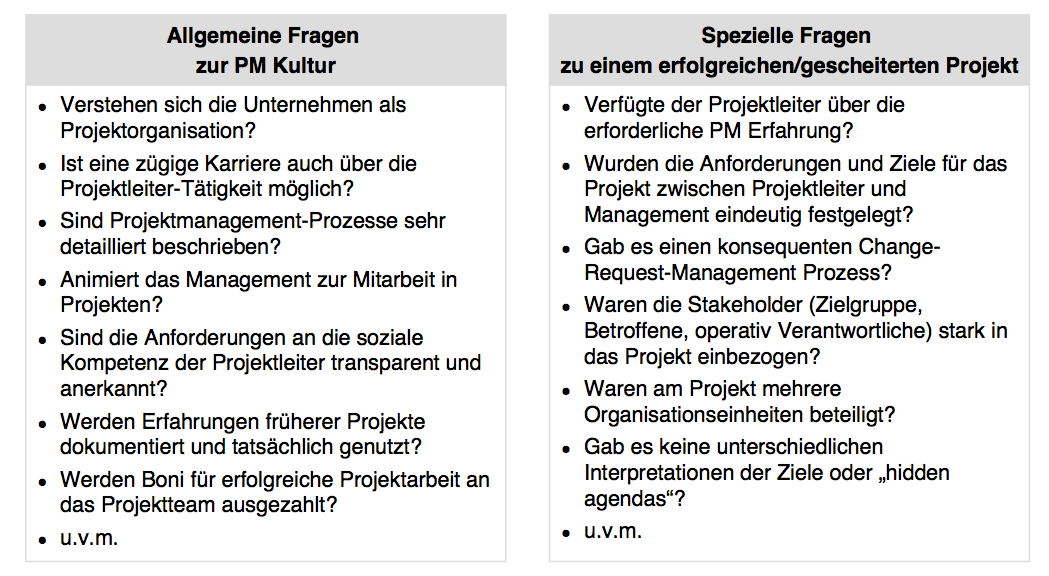
\includegraphics[width=0.9\textwidth]{img/fragen_gpm_studie}
		\caption{Fragen der GPM-Studie}
		\label{fragen_gpm_studie}	
	\end{center}
\end{figure}
\ 
\\
Für die vorliegende Ausarbeitung ist allerdings wesentlich interessanter was die Gründe für Erfolg oder Misserfolg von einzelnen Projekten sei. Dazu hat die GPM die teilnehmenden Unternehmen zu erfolgreichen und gescheiterten Projekten befragt. Für die Auswertung der Einzelprojekte wurde folgende Methodik angewandt\footnote{Vgl. \cite{GPM_Studie_2008, Seite 9}}:
\begin{itemize}
    \item{Fragen für erfolgreiche und gescheiterte Projekte sind identisch}
    \item{Für jede Frage wurde aus jeder Antwort ein Durchschnittswert ermittelt; jeweils für ''erfolgreiches Projekt'' und für ''gescheitertes Projekt''}
    \item{Durchschnittswert liegt zwischen 1 (''trifft überhaupt nicht zu'') und 5 (''Trifft voll und ganz zu'').}
    \item{Durchschnittswerte einer Frage wurden den beiden Projektkategorien (gescheitert, erfolgreich) gegenübergestellt}
    \item{Differenz soll Aufschluss über Faktoren für Projekterfolg liefern}
\end{itemize}
\
\\
Details zu den Ergebnissen finden sich in den Abschnitten \ref{ergebnis_pmk} (Projektmanagement-Kultur) und \ref{ergebnis_einzel} (Einzelprojekte)

\subsubsection{Teilnehmer}

Neben der Frage \textit{welche} Daten erhoben werden, muss auch geklärt werden, \texttt{wer} an der Studie teilgenommen hat. Dies waren 79 Unternehmen, überwiegend Organisationen mit mehr als 1000 Mitarbeitern und auch überwiegend Jahresumsätze von mehr als 1 Mrd. EUR (\textit{Vgl. siehe \cite{GPM_Studie_2008}, Seite 4}).\\
Es wurde versucht eine hohe Branchenvielfalt zu erreichen. Die Abbildung \ref{teilnehmer_gpm_studie} zeigt die prozentuale Teilnahme verschiedenster Branchen am Markt. Zu erwähnen sei noch, dass es einen hohen Anteil an von Unternehmen teilgenommen haben, die schon an früheren Studien der GPM oder PA-Group teilgenommen haben. 

\begin{figure}[H]
	\begin{center}
		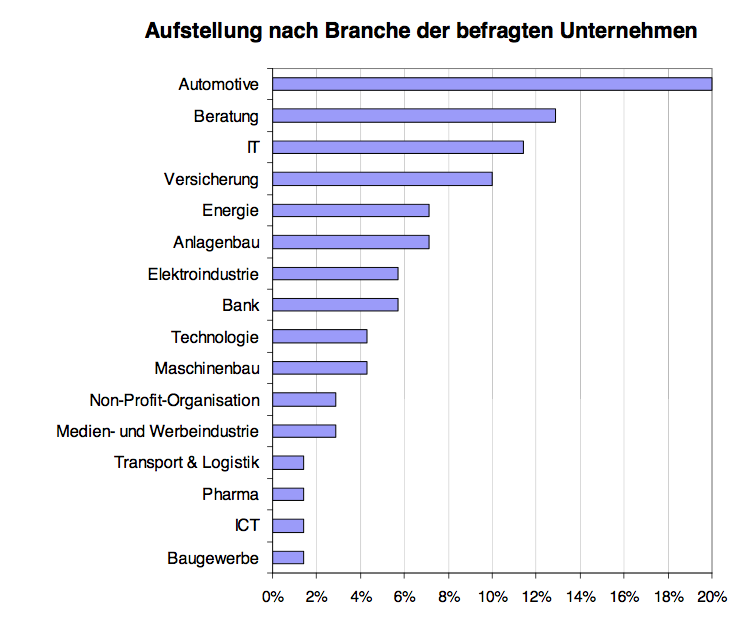
\includegraphics[width=0.9\textwidth]{img/teilnehmer_gpm_studie}
		\caption{Teilnehmer der GPM-Studie}
		\label{teilnehmer_gpm_studie}	
	\end{center}
\end{figure}

\subsubsection{Ergebnis der Projektmanagement-Kultur}
\label{ergebnis_pmk}
Das Ergebnis der Befragung der Projektmanagement-Kultur ist in Abbildung \ref{erfgebnis_gpm_studie_pmk} zu sehen. Fragen konnten nach einem Notensystem beantwortet werden, wobei 1 für ''Trifft gar nicht zu'' und 5 für ''Trifft voll und ganz zu'' einzusetzen sei. \\
Als \texttt{schwach} werden diejenigen Fragen bewertert die weniger als 3,5 in ihrem Durchschnittswert erzielt haben. Hier herrscht Optimierungsbedarf. 

\begin{figure}[H]
	\begin{center}
		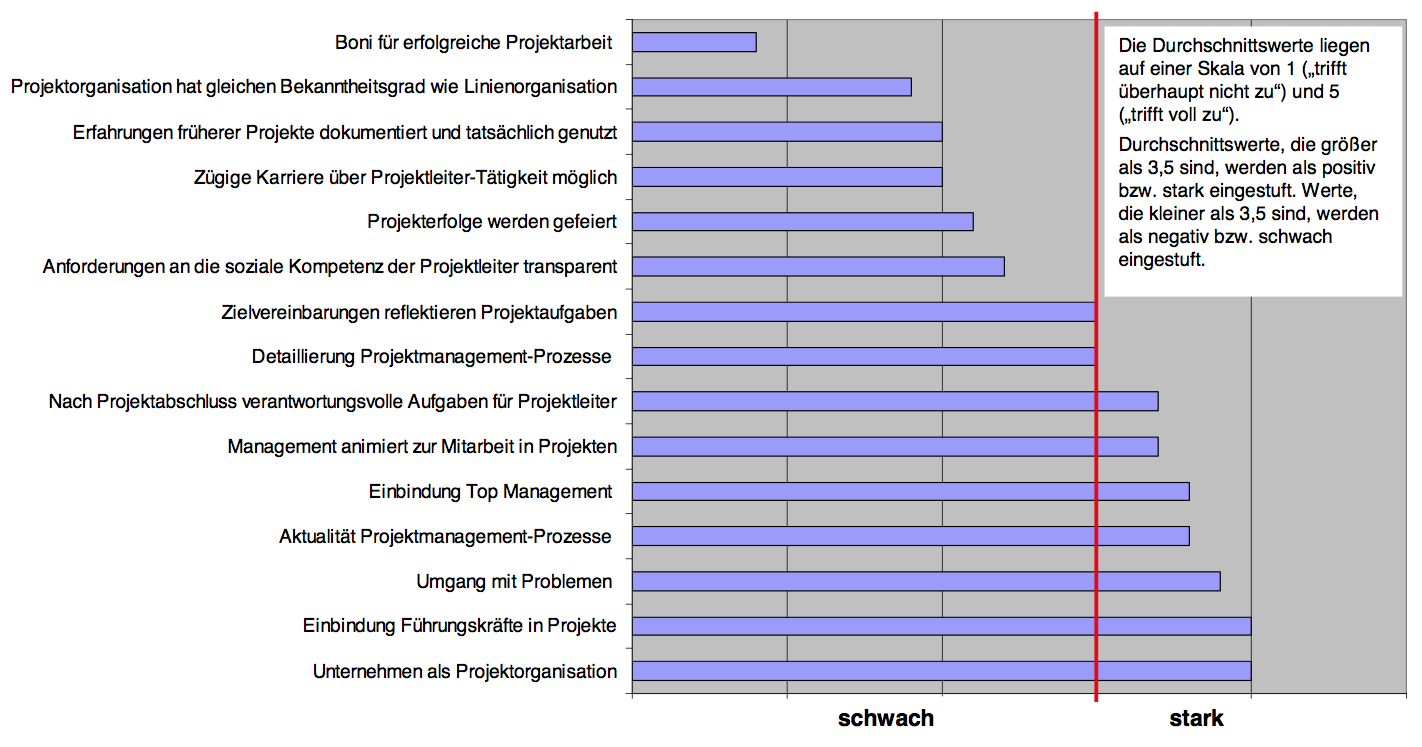
\includegraphics[width=1.0\textwidth]{img/ergebnis_gpm_studie_kultur}
		\caption{Ergebnis der GPM-Studie der Projektmanagement-Kultur}
		\label{erfgebnis_gpm_studie_pmk}	
	\end{center}
\end{figure}

%TODO: erweitern
Wie in Abbildung \ref{erfgebnis_gpm_studie_pmk} zu sehen ist werden zu wenig Boni für erfolgreiche Projektarbeit angeboten und auch zu wenig Karrierechancen als Projektleiter werden eingeräumt. Es fehlt also überwiegend ein Anreizsystem.\\
\\ 
Projektorganisation gleicht der Linienorganisation, nur zu wenig Erfahrung aus früheren Projekten werden dokumentiert und in anderen Projekten genutzt.

\subsubsection{Ergebnis Einzelprojekte}

Wie im Abschnitt \ref{erhobene_daten} beschrieben, galt es durch verschiedene Fragen an Projektbeteiligte von gescheiterten und erfolgreichen Projekten und Gegenüberstellungen dieser Fragen bestimmte Erfolgsfaktoren für Projekte zu ermitteln. Die Abbildung \ref{ergebnis_gpm_erfolgsfaktoren} zeigt die Top-10 der Gewichtungen der Antworten mit den größten Differenzen. Das rote Polygon zeigt die Gewichtung der gescheiterten Projekte und das blaue Polygon zeigt die Gewichtung der erfolgreichen Projekte. Zusammenfassend kann gesagt werden, dass den größten Erfolg eines Projekts die \texttt{Kommunikation}, das Aufstellen von \texttt{klaren Zielen} und die \texttt{Positio ndes Projektleiters} bestimmen und beeinflussen.

% TODO: Bild Erfolgsfaktoren, breite u. Höhe justieren
\begin{figure}[H]
	\begin{center}
		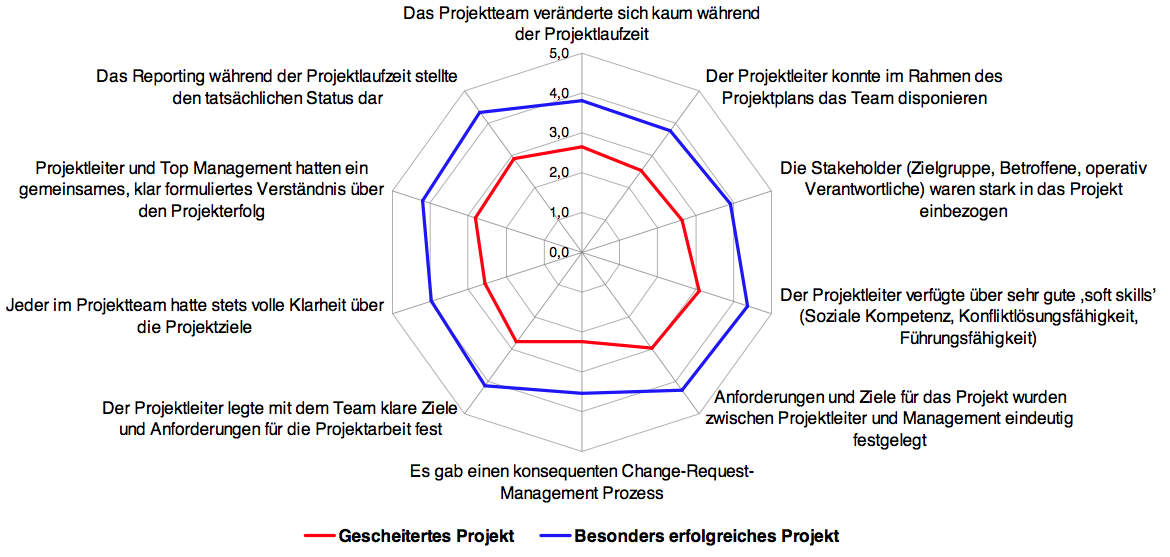
\includegraphics[width=1.1\textwidth]{img/ergebnis_erfolgsfaktoren}
		\caption{Die Erfolgsfaktoren in gescheiterten und erfolgreichen Projekten}
		\label{ergebnis_gpm_erfolgsfaktoren}	
	\end{center}
\end{figure}

\label{ergebnis_einzel}


\subsection{Auswertung der Ergebnisse}


% TODO: Gegenüberstellung
\pagebreak
\framebox{
	\colorbox{red!20}{
		\parbox{0.44\textwidth}{
Dolore te feugait nulla facilisi nam liber tempor cum soluta nobis eleifend option. Amet consectetuer adipiscing elit sed diam nonummy nibh euismod tincidunt ut laoreet. In iis qui facit eorum; claritatem Investigationes demonstraverunt lectores legere me. In vulputate velit esse molestie consequat vel illum dolore. Wisi enim ad minim, veniam quis nostrud exerci. Facer possim assum typi non habent claritatem insitam est usus legentis lius quod.
		}
	}
}
\framebox{
	\colorbox{green!20}{
		\parbox{0.44\textwidth}{
Dolore te feugait nulla facilisi nam liber tempor cum soluta nobis eleifend option. Amet consectetuer adipiscing elit sed diam nonummy nibh euismod tincidunt ut laoreet. In iis qui facit eorum; claritatem Investigationes demonstraverunt lectores legere me. In vulputate velit esse molestie consequat vel illum dolore. Wisi enim ad minim, veniam quis nostrud exerci. Facer possim assum typi non habent claritatem insitam est usus legentis lius quod.
		}
	}
}

\pagebreak

\pagebreak
\section{Probleme im Projektverlauf} 

Während des Projektverlaufs entstehen oft Probleme, die entweder schon in der Planungsphase entstanden sind und sich bisher durch das Projekt "geschlängelt" haben oder aber 

\subsection{Change Management}

\cite{profPM}
\cite{scriptPM}
\cite{chaosReportCriteria}

\pagebreak
\section{Kommunikationsprobleme}
\section{Projektziele}
\section{Rollenverteilung und Projektleiter}
\section{mangelnde Ressourcenverteilung}


\section{Fazit}

\pagebreak
\addcontentsline{toc}{section}{Literaturverzeichnis} % Eintrag ins Inhaltsverzeichnis
\bibliography{bib/bibliography}

\appendix

\end{document}
